% !TEX root = ../thesis-example.tex
%
\chapter{Einleitung}
\label{sec:intro}

%\cleanchapterquote{You can’t do better design with a computer, but you can speed up your work enormously.}{Wim Crouwel}{(Graphic designer and typographer)}

:TODO :NC

Keine bekannte Lebensform hat eine mit der menschlichen Sprache vergleichbar komplexe Form von Informationsaustausch entwickelt \cite{Rao}. Von selbst ergibt sich die Frage, ob und wie Sprache maschinell verarbeitet werden kann, um sie unter anderem zu interpretieren oder zusammenzufassen. Antworten auf diese Problemstellung liefert das Teilgebiet der Informatik \textit{Natural Language Processing} (Dt. Verarbeitung natürlicher Sprachen, kurz NLP). NLP gliedert sich in viele Teilbereiche: Strukturelle Analyse, Semantik, Phonetik und einige weitere. In dieser Arbeit konzentrieren wir uns auf einen wichtigen Bestandteil der strukturellen Analyse, dem korrekten Identifizieren von syntaktischen Rollen von Wörtern und Symbolen (\textit{Parts of Speech}, kurz POS), bezeichnet als \textit{POS-Tagging} \cite{Smith}.
\newline
Ein Algorithmus, der POS-Tagging betreibt (POS-Tagger), nimmt die Sprache in Textform an und gibt ihn üblicherweise mit Tags versehen wieder aus, wie Beispielsweise der Text
\newline \newline
\centerline{\textit{I like the blue house.}}
	
 zu folgendem verarbeitet wird:
\newline \newline
\centerline{\textit{I\textbf{\textbackslash PRONOUN} like\textbf{\textbackslash VERB} the\textbf{\textbackslash DET} blue\textbf{\textbackslash ADJ} house\textbf{\textbackslash NOUN} .\textbf{\textbackslash .}}}

Wie die Tatsächliche Ausgabe eines Taggers exakt formatiert wird und welche Tags auftreten, wird später angesprochen. Wichtiger ist hingegen, dass POS-Tagger diese Tags nicht garantiert korrekt wählen (siehe Abschnitt \ref{sec:intro:pos}). Es ist also von Interesse, deren Performance zu bewerten.


\section{Problemstellung dieser Arbeit}
\label{sec:intro:task}

Die Datenverarbeitungs-Plattform \textit{RapidMiner} :NC bietet im Rahmen der Erweiterung \textit{Text Processing} :NC Funktionen (\textit{Operatoren}), um Texte einzulesen und zu verarbeiten. NLP ist in RapidMiners Textverarbeitungs-Erweiterungen jedoch weitgehend noch nicht implementiert. Ziel dieser Arbeit ist es, in Form einer auf \textit{Text Processing} aufbauenden Erweiterung sowohl POS-Tagger zu implementieren, als auch ein Evaluationsrahmenwerk, mit dem deren Performance gemessen werden kann.

:TODO ?

Die implementierte Erweiterung liefert :TODO[anzahl] Tagging-Operatoren, :TODO[anzahl] Evaluationsoperatoren, ein spezialisiertes Übergabeformat für Tagging-Ergebnisse und eine Standardisierung für verwendete Tagsets :TODO[genauer?]. Gleichzeitig sind die Operatoren in ihrem Ein- und Ausgangsformat weitgehend kompatibel mit der Erweiterung \textit{Text Processing}.

\section{Part-of-Speech-Tagging allgemein}
\label{sec:intro:pos}

Betrachtet man das Wort \glqq like\grqq{} aus dem einleitenden Beispiel, dann fällt auf, dass es alternativ zum Verb \glqq mögen\grqq{} auch als Präposition \glqq wie\grqq{} interpretiert werden könnte, auch wenn intuitiv schnell erkennbar wird, dass letztere Variante falsch ist. Diese Uneindeutigkeit (\textit{Ambiguität}) ist das zentrale zu lösende Problem für POS-Tagger  \cite{Smith}; Im Gegensatz zum Menschen kann ein Algorithmus Ambiguitäten nicht intuitiv auflösen. Aus diesem Grund arbeiten POS-Tagger nicht zwingend vollständig korrekt.
\\
Während NLP viele andere Analyseaufgaben neben POS-Tagging zusammenfasst, sind diese bei moderneren und komplexeren NLP-Algorithmen nicht mehr strikt von POS-Tagging trennbar, wenn die Performance des Taggers maximiert werden soll :NC. Zusatzinformationen, die parallel erarbeitet werden können, wie z.B. die Satzstruktur (u.A. Identifizierung von Teilsätzen), können das auflösen von Ambiguitäten erheblich erleichtern. Zur Vereinfachung betrachten wir aber in dieser Arbeit nur POS-Tagging selbst, welches typischerweise in folgende zwei Arbeitsschritte unterteilt wird \cite{Smith}:

\paragraph{Sequenzialisierung:} Zuerst muss bestimmt werden, welche Teile des angegebenen Dokuments jeweils ein Tag erhalten. Hierzu wird jedes Wort und jedes zusammenhängende Satzzeichen als ein \textit{Token} ausgegeben. Die Reihenfolge der Wörter bleibt als Reihenfolge der Token hierbei erhalten. 
\paragraph{Tagging:} Mit Hilfe von statistischen, linguistischen und rechnerischen Methoden wird jedem Token ein POS-Tag zugewiesen. 

Es folgen noch ein paar weitere Erläuterungen und Definitionen:

\subsection{Tagset}
\label{sec:intro:pos:tagset}

Um einheitliche Verarbeitung und Vergleichbarkeit zu ermöglichen, werden die Tags in \textit{Tagsets} definiert, wie zum Beispiel dem des Penn-Treebank-Projekts \linebreak \cite{Web:PennBank} \cite{Paper:PennBank}.

\subsection{Korpus und Treebank}
\label{sec:intro:pos:corpus}

Als \textit{Korpus} bezeichnet man eine simple Ansammlung von Text. Der \textit{WSJ-Korpus}  :NC beispielsweise ist eine Sammlung von Artikeln der Nachrichtenartikel des \textit{Wall Street Journal}.
\\
Korpora, die zu Token-Ketten sequenzialisiert wurden und deren Token mit (POS-) Tags versehen wurden, werden als annotierte Korpora oder \textit{Treebanks} bezeichnet. Zusätzlich ist eine Treebank mit anderen Informationen wie der Satzstruktur versehen, diese sind hier aber nicht weiter relevant. Treebanks sind in der Regel zu nahezu 100\% korrekt annotiert. Ist dies der Fall, spricht man auch von einem \textit{Goldstandard}. Da Goldstandards manuell korrigiert werden, können seltene Fehler auftreten. Diese sind allerdings zu wenige, um als relevant angesehen zu werden. :NC

\subsection{Evaluationsmetriken}
\label{sec:intro:pos:metrics}

Um die Performance eines Taggers zu bewerten, müssen Metriken eingeführt werden. Diese entstehen aus Vergleichen zwischen annotierten Korpora und den Tagging-Ergebnissen. Es folgt eine kurze Auflistung gängiger Wege, die Ergebnisqualität eines Taggers zu berechnen:

\subsubsection{Per-Tag-Accuracy}

Die Per-Tag-Accuracy (ab hier nur \textit{Accuracy}) ist die wichtigste und einfachste Form der Bewertung eines Taggers. Sie ist definiert als \cite{Rao} :

\[ \frac{\# \: korrekter \:  Tags}{\# \: aller \:  Token} \]

\subsubsection{Per-Sentence-Accuracy}

Analog zur Accuracy pro Tag kann auch Accuracy pro Satz definiert werden:

\[ \frac{\# \: vollständig \: korrekter \:  Sätze}{\# \: aller \:  Sätze} \]

Hierzu müssen jedoch über Wort-Sequenzen hinaus auch Satz-Sequenzen definiert werden. In der Evaluation in Abschnitt \ref{sec:related:stanford} wurde dies ebenfalls berücksichtigt. :TODO

\subsubsection{Confusion Matrix und daraus resultierende Metriken}
Konzentrieren wir uns auf bestimmte Tags (Labels), können wir genauere Aussagen Treffen
(Für allgemeine Definitionen siehe \cite{Rao}, für mehrklassige Klassifizierungsprobleme siehe \cite{Web:rxnlp}). Zuerst bilden wir die \textit{Confusion Matrix}. In Abbildung \ref{fig:intro:pos:metrics:confusion} befindet sich ein Beispiel dafür. In dieser Matrix wird gegenübergesetzt, wie viele Labels aus dem Goldstandard als welche Labels vom Tagger vorhergesagt wurden.
\begin{description}

\item[True Positives] für Label X (kurz TP(X)) sind Vorhersagen, die dem Goldstandard entsprechen (in der Abbildung Gelb markiert).
\item[False Positives] (FP(X)) sind alle Vorhersagen X, die dem Goldstandard widersprechen.
\item[True Negatives] (TN(X)) sind alle Vorhersagen, die nicht X sind, und auch im Goldstandard nicht X lauten.
\item[False Negatives] (FN(X)) sind alle Vorhersagen, die nicht X sind, im Goldstandard aber X.
\end{description}

\begin{figure}[htb]
	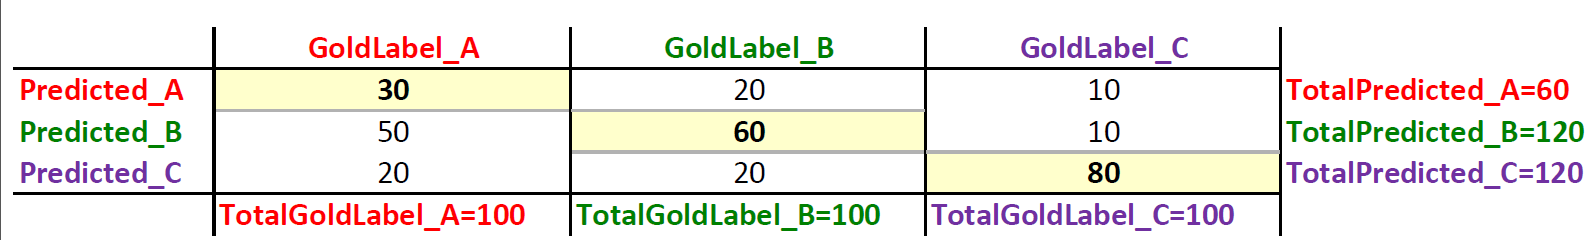
\includegraphics[width=\textwidth]{gfx/multi-class-confusionmatrix.png}
	\caption{Beispiel für eine Confusion Matrix für Labels A, B, C. Entnommen von \cite{Web:rxnlp}}
	\label{fig:intro:pos:metrics:confusion}
\end{figure}

Daraus lassen sich Precision(Wie viele der Vorhersagen X waren korrekt?), Recall(Wie viele X im Goldstandard wurden korrekt erkannt?) und der F1-Score(auch F-Score, harmonisches Mittel aus Precision und Recall) berechnen:
\[ Precision(X) \: = \: \frac{TP(X)}{TP(X)+FP(X)}\: = \: \frac{TP(X)}{Vorhergesagte\:X} \]
\[ Recall(X) \: = \: \frac{TP(X)}{TP(X)+FN(X)} \: = \: \frac{TP(X)}{X\:im\:Goldstandard} \]
\[ F1\mbox{-}Score \: = \: 2*\frac{Precision(X)*Recall(X)}{Precision(X)+Recall(X)} \]

Für alle drei dieser Metriken steht der Wert 1 für vollständig richtig und 0 für vollständig falsch.


\section{Aufbau der Arbeit}
\label{sec:intro:structure}

\begin{description}

\item[Kapitel \ref{sec:related}] betrachtet einige Implementierungen von Part-of-Speech-Taggern und deren Evaluation in anderen Projekten.
\item[Kapitel \ref{sec:concept}] erläutert die Methodik und behandelten Probleme in diesem Projekt.
\item[Kapitel \ref{sec:impl}] beschreibt detailliert die Implementierung und deren Zielsetzung der RapidMiner-Erweiterung.
\item[Kapitel \ref{sec:eval}] führt Evaluationen der implementierten POS-Tagger anhand eines gewählten Goldstandards auf.

\end{description}

